\section{Magnetic Design}

Firstly, the shape of the transformer core is selected as an E-core. Since E-cores can be winded better than toroid cores. To have enough turn numbers on both primary and secondary side, KOOL MU 2510 E CORE(00K2510E090) is selected. Cross-section area of the core is important for turn numbers and core area of the KOOL MU 2510 E CORE is small enough to have 10 turns on the primary side. Parameters of the chosen E-core is given below:

\begin{align}
    A_e &= 35\;mm^2\;(Cross\; Sectional\; Area)\\ l_e &= 48.5\; mm \;(Magnetic\;Path\; Length) \\\mu_c &= 90\; (Relative \;Permeability) \\ B_c &= 1\; T \;(Saturation\; Flux\; Density) \\ Weight &= 5.9\; g\; and\; V_e=1870\; mm^3 \;(Volume) 
\end{align}

According to chosen core secondary turn numbers was calculated.

\begin{align}
    N_S&=\frac{L_P\times I_{peak}}{n\times B_m \times A_e}\\
    N_S&=\frac{28.67\times 10^{-6} \times 10.8 }{1.9 \times 1 \times 35 \times 10^{-6}}=5.2 \;turns
\end{align}

Ratio of the primary turn numbers to secondary turn numbers is calculated, so primary turn number is given below;

\begin{align}
    N_P= n\times N_S = 1.9 \times 5.2 = 10\; turns
\end{align}

In this flyback converter design, UCC28740 analog controller is chosen to control the output voltage and current. To supply V$CC$(7.75V) to UCC28740 analog controller, there is required auxiliary winding come from the transformer. The turn number of the auxiliary winding is calculated below:

\begin{align}
    N_{VCC}= \frac{V_{CC}}{V_O+V_F}\times N_S = \frac{7.75}{12+0.7}\times N_S= 3 \;turns
\end{align}

$$ N_{VCC}= 3\;turns $$

There is a core gap on the E-core. Core gap is crucial because magnetic flux intensity can be controlled by the core gap. If there is smaller gap than required, the core can be saturated and transformer could not work properly. Also the other components of the flyback converter can be damaged due to overload. Required core gap is calculated to have optimum magnetic design. Calculation of the core gap is given below:

\begin{align}
    gap=\frac{\mu_0\times N_P{^2}\times A_e }{L_P}-\frac{I_e}{\mu_c}
    \label{eqn:gap}
\end{align}

$$ gap = \frac{1.256\times 10^{-6}\times 10{^2}\times 35\times 10^{-6}}{28.67\times 10^{-6}}-\frac{48.5\times 10^{-3}}{90}=1.35\times 10^{-3}\;m $$

$$ gap = 1.35\times 10^{-3}\;m = 1.35\;mm $$

To check the calculated values given equations is done. Magnetic flux intensity is crucial, since if it is higher than the saturation level of the core, saturation level of the chosen core is 1 Tesla.

\begin{align}
    B=\frac{\mu_0\times N_P\times I_P}{\frac{I_e}{\mu_c}+gap}&=\frac{1.256\times 10^{-6}\times 10\times 10.8}{\frac{48.5\times 10^{-3}}{90}+3.85\times 10^{-3}}=0.95\\
    V_r&=\frac{N_P}{N_S}\times (V_O+V_F)=24.13 V
\end{align}

0.95 Tesla is lower than saturation level of the core so it is acceptable. Also duty ratio must be lower than 0.53. To check duty ratio of the design, D is calculated below:

\begin{align}
    D=\frac{V_r}{V_r+V{_dc(min)}}=0.5
\end{align}

\subsection{Transformer Selection}

According to the design calculations and simulation results of the ideal Flyback Converter circuit presented in the Simulation Report, the peak current of the transformer is equal to 10.8 Ampere, turn ratio of the transformer is 1.9:1, primary turn number of transformer is determined as 10, and the secondary turn number is equal to 5. Transformer primary side voltage is between 24-48 V which is input voltage range. To obtain the required turn numbers, the cross-section area of the core must be smaller than 40 $mm^2$ and core saturation density of the available cores B = 1 Tesla. According to the required cross-section area range, KOOL MU 2510 E core is chosen. The cross-sectional area of the chosen core is 38.5 $mm^2$. The effective magnetic path length of the core is 48.5 $mm$. The permeability of the core is given as 90$\mu$.

$$ turns\; ratio = 1.9 \approx 2 $$

$$ N_P = 10\; turns $$

$$ N_S = 5\; turns $$

The Figure \ref{fig:Permeability} below shows the detailed dimensions and the permeability and inductance per turn squared values of the KOOL MU 2510 E core.

\begin{figure}[!h]
\centering
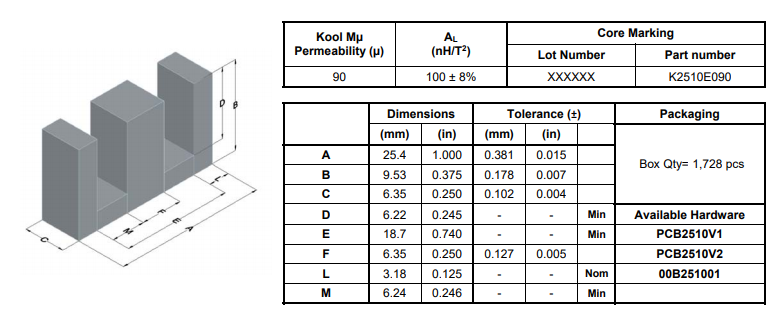
\includegraphics [width=1\textwidth]{figures/core.png}
\caption{Detailed dimensions of the E core and relative permeability of core }
\label{fig:Permeability}
\end{figure}

The cross-sectional area is important to decide turn numbers and the air gap between E cores. Information about cross-sectional area and magnetic path length is given Figure \ref{fig:Csa}. As can be seen from equation \eqref{eqn:gap2}, the gap is directly affected by path length and relative permeability, so both the magnetic path length and the relative permeability are also crucial for the magnetic design.

\begin{align}
    gap=\frac{\mu_0\times N_P^2 \times A_e}{L_P}-\frac{l_e}{\mu_c}
    \label{eqn:gap2}
\end{align}
Magnetic flux density of the core can be calculated by given formula;
\begin{align}
    B=\frac{\mu_0\times N_P\times A_e}{\frac{l_e}{\mu_c}+gap}
    \label{eqn:fluxB}
\end{align}

As seen from equation \eqref{eqn:fluxB}, magnetic flux density depends on the cross-sectional area, magnetic path length and relative permeability of the core. The cross-sectional area and relative permeability are limited since the core can be saturated. Magnetic flux density is inversely proportional with air gap length and magnetic path length. As can be seen from Figure \ref{fig:SFD}, saturation flux density of the KOOL MU magnetic cores is equal to 1 Tesla. The core shape, cross-sectional area and magnetic path length are chosen according to the saturation flux density of the KOOL MU magnetic core, which is 1 Tesla.

$$ B_{sat} = 1\;Tesla $$

\begin{figure}[!h]
\centering
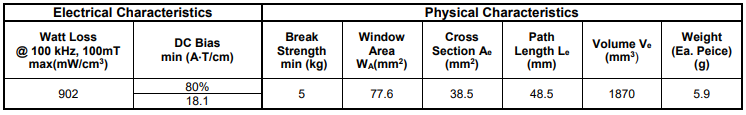
\includegraphics [width=1\textwidth]{figures/area vs.png}
\caption{Cross sectional area and Path Length of core }
\label{fig:Csa}
\end{figure}
\begin{figure}[H]
\centering
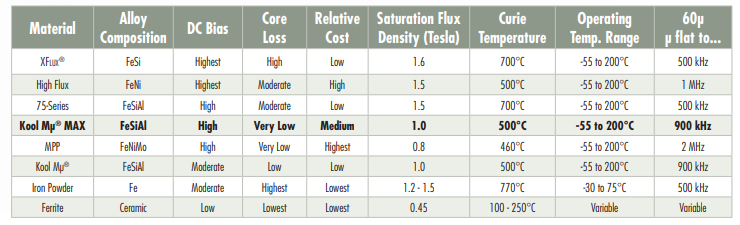
\includegraphics [width=1\textwidth]{figures/permeability.png}
\caption{Saturation Flux Densities of various magnetic cores }
\label{fig:SFD}
\end{figure}

\subsection{Cable Selection}

In order to make the proper cable selection for the designed Flyback Converter circuit, we, first of all, need to determine the skin depth at the selected switching or operating frequency.

$\delta$= Skin Depth\\
$\rho$= Resistivity of Material\\
$\mu_r$= Relative Permeability of Cable\\
$\mu_0$= Permeability Constant = $4\pi\times 10^{-7}$\\
$f_s$ = switching frequency = 45 kHz \\

Then, the skin depth is given by the following formula in equation \eqref{eqn:skin}.

\begin{align}
    \delta=\sqrt{\frac{\rho}{\pi\times f\times \mu_r\times \mu_0}}
    \label{eqn:skin}
\end{align}

For copper cables, the formula in equation \eqref{eqn:skin} can be reduced to the following simplified for as given in equation \eqref{eqn:skin2}, below.

\begin{align}
    \delta=\frac{7.5}{\sqrt{f_s}}\; cm = \frac{75}{\sqrt{f_s}}\; mm
    \label{eqn:skin2}
\end{align}

Then, we can compute the skin depth at the switching frequency of $f_s$ = 45 kHz, as follows:

$$ \delta=\frac{75}{\sqrt{45000}}\; mm $$

$$ \delta= 0.3535\; mm $$

At 45 kHz switching frequency, skin depth of copper cable is equal to 0.3535 mm.

Furthermore, we also need to determine the maximum RMS current that flows through the primary or the secondary winding terminals of the transformer in order to make the cable selection with the proper dimensions and sizes.

Since the voltage ratings of the output side (15 V) of the designed Flyback Converter is less than the input side voltage ratings (24-48 V), the output current ratings of the converter is higher than the input current ratings. In other words, the secondary side current ratings of the transformer is higher than the primary side current ratings. Therefore, for the appropriate cable selection, we need to consider the maximum RMS current rating on the secondary (output) side of the transformer.

The average output current of the Flyback Converter can be determined from the following power relation.

\begin{align}
    P_{out} = V_{out}I_{out}
    \label{eqn:power}
\end{align}

If we substitute the average output power of 60 W and the average output voltage of 15 V into the above equation \eqref{eqn:power}, we can obtain the average output current as 4 A, as follows:

$$ I_{out} = \frac{P_{out}}{V_{out}} = \frac{60}{15} = 4\;A $$

$$ I_{out} = 4\;A $$

The maximum ripple in the secondary side current of the transformer is equal to the maximum current ripple on the output diode of the Flyback Converter topology. The maximum current ripple in the diode current is measured as 19.42 A in the simulations with the ideal Flyback Converter circuit in Simulink as also stated in the Simulation Report.

$$ \Delta i_{D,max} = 19.42\;A $$

After computing the average current and the maximum ripple current values in the transformer secondary side, we can, finally, calculate the maximum RMS current value on the secondary side of transformer by using the following relation given in equation \eqref{eqn:rms_current}.

\begin{align}
    I_{sec,RMS} = \sqrt{I_{out}^2 + (\frac{\Delta i_{D,max}}{2})^2}
    \label{eqn:rms_current}
\end{align}

Hence, if we substitute the computed current values into the equation \eqref{eqn:rms_current}, the maximum RMS current value of the secondary side current of the transformer is obtained as follows:

$$ I_{sec,RMS} = \sqrt{4^2 + (\frac{19.42}{2})^2} = \sqrt{16 + 94.28} = \sqrt{110.28} = 10.5\;A\; (RMS) $$

$$ I_{sec,RMS} = 10.5\;A\; (RMS) $$

Hence, the analytical result for the secondary side RMS current value of the transformer is obtained as 10.5 A (RMS).

In the simulations with the ideal Flyback Converter circuit in Simulink, the maximum RMS current at the secondary side of the transformer is measured as 8.138 A (RMS).

$$ I_{sec,RMS} = 8.138\;A\; (RMS) $$

This current value is close to the above analytically computed RMS current value of 10.5 A. However, since the analytical equation that is utilized to compute the secondary RMS current value is not exactly correct, and does not give exact results, we will use the RMS current value obtained from the simulations of the ideal Flyback Converter circuit in Simulink in order to make the cable selection for the transformer.

Hence, the secondary side maximum RMS current of the transformer is obtained as 8.138 A (RMS).

The maximum current density that a copper cable can carry is given as J = 4 $A/mm^2$.

Then, the minimum required cable cross-sectional area is found as follows:

\begin{align}
    A_{conductor} = \frac{I_{sec,RMS}}{J}
    \label{eqn:area_cond}
\end{align}

Then, the minimum required conductor area for the selected cable is found as follows by substituting the necessary parameters into the equation \eqref{eqn:area_cond}.

$$ A_{conductor} = \frac{8.138}{4} = 2.0345\;mm^2 $$

$$ A_{conductor} = 2.0345\;mm^2 $$

However, since this required conductor area value is large, and since it will result in a very thick and large cable selection, we decided to use some cables in parallel in order to reduce the current stress over each cable, and hence also help us to select much thinner and small cables. Furthermore, using parallel cables also provides the benefit of reduced copper resistances and hence copper losses. One another advantage of using parallel cables is that they help to achieve the optimal wounding geometry around the transformer window area, which helps to reduce the leakage fluxes, proximity and skin effect disruptions.

As a result, we decided to utilize 4 cables in parallel for the primary and secondary windings of the transformer.

This, in result, reduces the minimum required conductor area for the selected cable to one fourth of the previously computed minimum required conductor area value.

Hence, the new minimum required conductor area with using 4 cables in parallel is obtained as follows:

$$ A_{conductor} = \frac{2.0345}{4} = 0.508625\;mm^2 $$

$$ A_{conductor} = 0.509\;mm^2 $$

As a result, we can select cable AWG\#19 considering the given conductor area limitations.

\textbf{Selected Cable: }AWG\#19
The parameters of the selected cable is given below.

\begin{itemize}
    \item The diameter of the cable: 0.91186 mm
    \item The conductor cross-sectional area of the cable: 0.653 $mm^2$
    \item Ohms per km: 26.40728 \ohm/km
\end{itemize}

After making the cable selection, we can finally compute the fill factor of the designed transformer for the Flyback Converter.

First of all, we need to compute the total conductor area that fills the window area of the designed transformer. In order to compute the total conductor area, we, first of all, need to multiply the cross-sectional area of the selected cable with the number of paralleled cables, which is 4. Then, the total conductor area is obtained by multiplying the above computed value with the total number of turns of the primary and the secondary side of the transformer.

\begin{align}
    \sum A_{conductor} = (N_P + N_S)\times A_{conductor}\times 4
    \label{eqn:total_area}
\end{align}

Then, the total conductor area is obtained as follows by substituting the necessary parameters into the equation \eqref{eqn:total_area} above.

$$ \sum A_{conductor} = (10 + 5)\times 0.653\times 4 = 15\times 0.653\times 4 = 39.18\;mm^2 $$

$$ \sum A_{conductor} = 39.18\;mm^2 $$

Finally, the fill factor can be obtained by using the following relation.

\begin{align}
    fill\;factor = \frac{\sum A_{conductor}}{A_{window}}
    \label{eqn:fill_factor}
\end{align}

The window area of the selected core is equal to 77.62 $mm^2$ as given in its datasheet, as shown in Figure \ref{fig:SFD} above.

As a result, we can compute the fill factor for the designed transformer by substituting the above parameters into equation \eqref{eqn:fill_factor}, as follows.

$$ fill\;factor = \frac{39.18}{77.62} = 0.5 $$

$$ fill\;factor = 0.5\; (50\%) $$

This value is quite reasonable since it shows that our window area utilization is quite good with nearly 50\%. Furthermore, it is also
lower than the practical upper limit of 0.6 (or 60\%) for round copper cables. This value of fill factor shows that we are utilizing nearly the half of the window area of the designed transformer, which is a quite reasonable design.

Next, we nee to compute the DC and AC resistances of the transformer windings.

First of all, we start by computing the DC resistances of the transformer primary and secondary windings.

The mean length per turn value for the selected core is computed as follows by using the core dimensions given in its datasheet as shown in Figure \ref{fig:Permeability} above.

\begin{align}
    MLT = \pi(\frac{E + F}{2})
    \label{eqn:mlt}
\end{align}

Then, the mean length per turn value for the selected core is obtained as follows by substituting the necessary dimension values in equation \eqref{eqn:mlt} from its datasheet.

$$ MLT = \pi \times (\frac{18.7 + 6.35}{2}) = \pi \times 12.525 = 39.348\; mm $$

$$ MLT = 39.348\; mm $$

Next, the total length of the primary winding is obtained by multiplying the MLT value with the primary number of turns $N_P$.

\begin{align}
    Length_{Pri} = MLT\times N_P
\end{align}

Hence, the total length of the primary winding is found as follows:

$$ Length_{Pri} = 39.348\times 10 = 393.48\; mm $$

We can round this value up to 400 mm.

$$ Length_{Pri} \approx 400\; mm $$

Similarly, we can compute the total length of the secondary winding of the transformer by multiplying the MLT value with the secondary number of turns $N_S$.

\begin{align}
    Length_{Sec} = MLT\times N_S
\end{align}

Hence, the total length of the secondary winding is found as follows:

$$ Length_{Sec} = 39.348\times 5 = 196.742\; mm $$

We can round this value up to 200 mm.

$$ Length_{Sec} \approx 200\; mm $$

In order to compute the DC resistances of the primary and the secondary windings, we need to multiply the resistance per mm ratio of the selected cable with calculated primary and secondary winding lengths. Finally, the DC resistance values of the primary and secondary windings are obtained by dividing the result by 4 since we used 4 cables in parallel in the construction of the primary and the secondary windings.

The per km resistance of the selected cable is given as:

$$ R = 26.40728\; \ohm / km  $$

Then, the per mm resistance of the selected cable is obtained as:

$$ R = 26.40728\times 10^{-6}\; \ohm / mm  $$

Finally, the DC resistance of the primary winding is computed as follows:

\begin{align}
    R_{DC,pri} = \frac{R\times Length_{Pri}}{4} 
\end{align}

$$ R_{DC,pri} = \frac{26.40728\times 10^{-6}\times 400}{4} = 2.64\;m\ohm $$

$$ R_{DC,pri} = 2.64\;m\ohm $$

Similarly, the DC resistance of the secondary winding is computed as follows:

\begin{align}
    R_{DC,sec} = \frac{R\times Length_{Sec}}{4} 
\end{align}

$$ R_{DC,sec} = \frac{26.40728\times 10^{-6}\times 200}{4} = 1.32\;m\ohm $$

$$ R_{DC,sec} = 1.32\;m\ohm $$

Now, after computing the DC resistances of the primary and the secondary winding, we need to compute the AC resistances of the primary and the secondary winding.

For that, first of all, we need to compute the effective cross-sectional area of the cables at the operating (switching) frequency of $f_s$ = 45 kHz.

The effective cross-sectional area of the cables is computed as follows by using the computed skin depth value.

\begin{align}
    A_{effective} = \pi\times ((\frac{D}{2})^2 - (\frac{D}{2} - \delta)^2)
\end{align}

$$ A_{effective} = \pi\times ((\frac{0.91186}{2})^2 - (\frac{0.91186}{2} - 0.3535)^2) $$

$$ A_{effective} = \pi\times ((0.45593)^2 - (0.10238)^2) = 0.620\;mm^2 $$

$$ A_{effective} = 0.620\;mm^2 $$

Finally, the AC resistances of the primary and the secondary winding are obtained as follows:

For primary:

\begin{align}
    R_{AC,pri} = R_{DC,pri}\times \frac{A_{conductor}}{A_{effective}}
\end{align}

$$ R_{AC,pri} = 2.64\times \frac{0.653}{0.620} $$

$$ R_{AC,pri} = 2.78\;m\ohm $$

For secondary:

\begin{align}
    R_{AC,sec} = R_{DC,sec}\times \frac{A_{conductor}}{A_{effective}}
\end{align}

$$ R_{AC,sec} = 1.32\times \frac{0.653}{0.620} $$

$$ R_{AC,sec} = 1.39\;m\ohm $$

We can tabulate the computed AC resistance values as shown in the following table.

\begin{table}[H]
    \centering
    \caption{AC Coil Resistances}
    \begin{tabular}{|c|c|}
    \hline
\textbf{Parameter}   & \textbf{Value}             \\ \hline
$R_{AC,pri}$ & 2.78\;m\ohm \\ \hline
$R_{AC,sec}$ & 1.39\;m\ohm \\ \hline
    \end{tabular}
    \label{tab:resistance_ac}
\end{table}